We document here the behaviour of variants of pypei on a testbed
problem.

\hypertarget{testbed-problem}{%
\section{Testbed problem}\label{testbed-problem}}

We take a standard SIR model:

\[\begin{aligned}
S' &= -\beta SI/N \\
I' &= \beta SI/N - \alpha I\\
R' &= \alpha I\\
N &= S + I + R\\
\end{aligned}\]

and solve it forward it time over \(t \in [0, 20]\) for the parameters
\(\theta_{true}\) and initial conditions \({y_0}_{true}\) to get a true
solution \(y_{true}\):

\[\begin{aligned}
\theta_{true} = [\beta_{true}, \alpha_{true}] &= [1.3, 0.2]\\
{y_0}_{true} = [{S_0}_{true}, {I_0}_{true}, {R_0}_{true}] &= [999, 1, 0]
\end{aligned}\]

We generate (noisy) data \(y\) by observing only the states \([S, R]\)
over a time period \(t \in [0, 7]\), which we encapsulate in an
observation function, \(g(\cdot)\), subject to Poisson noise:

\[y \sim \text{Poisson}(g(y_{true}))\]

\hypertarget{standard-variant}{%
\section{Standard variant}\label{standard-variant}}

We fit the objective function
\(H_{standard} = -2\log\mathcal{L}_{standard}\):

\[
H_{standard} = \lVert L(y - g(\Phi c))\rVert^2 + \lVert W(D\Phi c - f(\Phi c, \theta)) \rVert^2 - 2\log{|L|} - 2\log{|W|}
\] where
\[L = \frac{1}{\sigma_L} \mathbb{I},\qquad W = \frac{1}{\sigma_W} \mathbb{I}\]
and we define the weights:
\[w = \left[\frac{1}{\sigma_L}, \frac{1}{\sigma_W}\right]\]

We solve this iteratively:

\begin{enumerate}
\def\labelenumi{\arabic{enumi}.}
\tightlist
\item
  Set the iteration number \(i=0\).
\item
  Set initial guess \(c^{(0)}, \theta^{(0)}\) and initial weights
  \(w^{(0)}\).
\item
  Minimise \(H_{standard}\) over \(c, \theta\) for given weights
  \(w^{(i)}\) \(\to c^{(i+1)}, \theta^{(i+1)}\).
\item
  Minimise \(H_{standard}\) over \(w\) for given
  \(c^{(i+1)}, \theta^{(i+1)}\) \(\to w^{(i+1)}\).
\item
  If \(i\) \textless{} maximum iterations, set iteration number
  \(i \gets i+1\) and return to step 2.
\end{enumerate}

We shortcut step 4 by instead doing:

\(w^{(i+1)} \gets s(c^{(i+1)}, \theta^{(i+1)})\)

where \(s(c, \theta)\) = \(\sqrt{\frac{n}{r(c, \theta)}}\) and \(r\) is
the residual function, \(n\) the length of \(r(c, \theta)\).

In this case
\(r(c, \theta) = \left[y - g(\Phi c), \;D\Phi c - f(\Phi c, \theta)\right]\).
We justify this by stating that this is the `optimal' solution via
solution of the KKT conditions, once \(r\) is known (assuming there are
no constraints imposed on the problem, which is not necessarily true).

Here, we `absorb' scaling into the covariance matrices, but because we
do not optimise for them directly, we don't get the proper scalings.

\hypertarget{results}{%
\subsection{Results}\label{results}}

We use initial weights \([1, 1]\), and initial guesses
\(\sim \text{Poisson}(1000)\). We have to terminate the iteration early,
at iteration \(i=1\) where \(w=[0.05, 0.49]\), and recover parameter
estimates \(\beta = 1.19, \alpha = 0.19\). Runtime is 8.85s for 4
iterations.

\begin{figure}
\centering
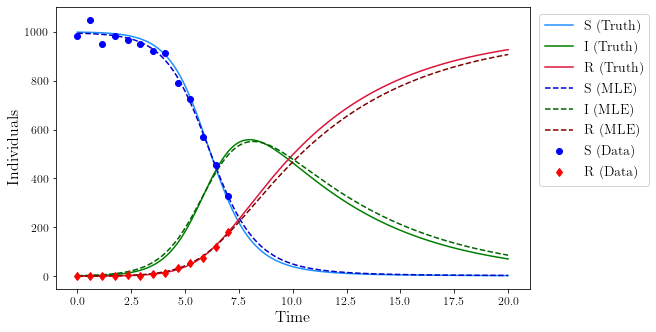
\includegraphics{img/standard_fit_iter1.png}
\caption{Fit to \(H_{standard}\) at iteration \(i=1\)
(\(\beta=1.19, \alpha=0.19\))}
\end{figure}

The model weights grow at each iteration, we can see that it leads to
underfits.

\begin{figure}
\centering
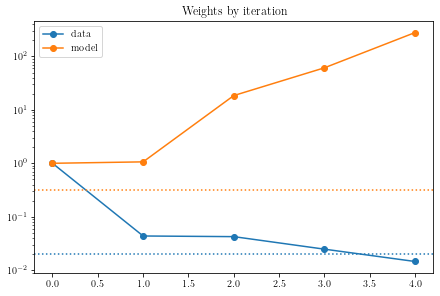
\includegraphics{img/standard_weights.png}
\caption{Weights for each iteration, solving \(H_{standard}\)}
\end{figure}

Iteration 0 seems well fit. By iteration 2, the fit is already degraded,
and by iteration 3, the estimate is very underfit.

\begin{figure}
\centering
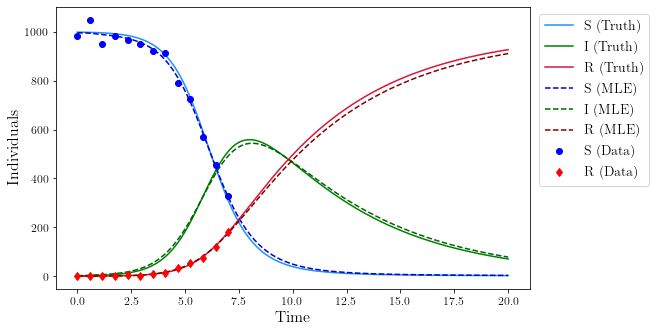
\includegraphics{img/standard_fit_iter0.png}
\caption{Fit to \(H_{standard}\) at iteration \(i=0\)
(\(\beta=1.20, \alpha=0.19\))}
\end{figure}

\begin{figure}
\centering
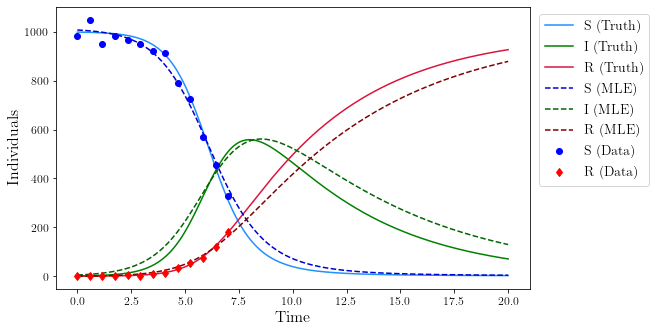
\includegraphics{img/standard_fit_iter2.png}
\caption{Fit to \(H_{standard}\) at iteration \(i=2\)
(\(\beta=0.84, \alpha=0.13\))}
\end{figure}

\begin{figure}
\centering
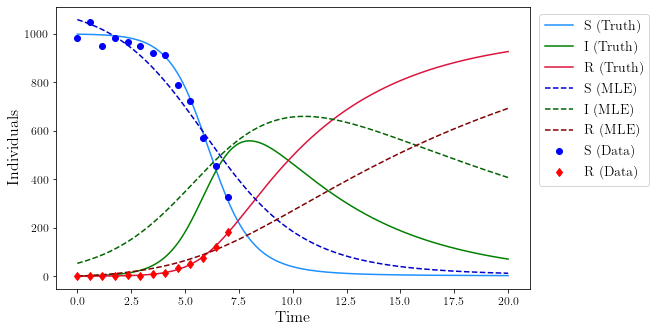
\includegraphics{img/standard_fit_iter3.png}
\caption{Fit to \(H_{standard}\) at iteration \(i=3\)
(\(\beta=0.55, \alpha=0.08\))}
\end{figure}

\hypertarget{delta-t-variant}{%
\section{Delta-t variant}\label{delta-t-variant}}

We fit the objective function
\(H_{\Delta t} = -2\log\mathcal{L}_{\Delta t}\):

\[
H_{\Delta t} = \lVert L(y - g(\Phi c))\rVert^2 + \lVert W(\,\sqrt{\Delta t}(D\Phi c - f(\Phi c, \theta))\,) \rVert^2 - 2\log{|L|} - 2\log{|W|}
\] where
\[L = \frac{1}{\sigma_L} \mathbb{I},\qquad W = \frac{1}{\sigma_W} \mathbb{I}\]
and we define the weights:
\[w = \left[\frac{1}{\sigma_L}, \frac{1}{\sigma_W}\right]\]

Essentially, we introduce a scaling \(\Delta t\) into the
\emph{residual} function. This fixes the consistency problem with the
SDE interpretation, that is not explicitly addressed in the standard
variant (with shortcut).

\hypertarget{results-1}{%
\subsection{Results}\label{results-1}}

We use initial weights \([1, 1]\), and initial guesses
\(\sim \text{Poisson}(1000)\). We have to terminate the iteration early,
at iteration \(i=1\) where \(w=[0.05, 0.49]\), and recover parameter
estimates \(\beta = 1.19, \alpha = 0.19\). Runtime is

\begin{figure}
\centering
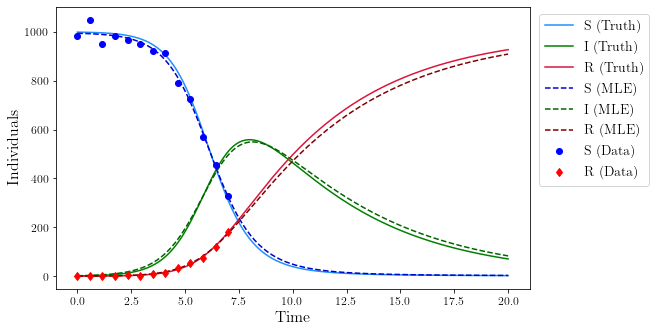
\includegraphics{img/dtvariant_fit_iter1.png}
\caption{Fit to \(H_{\Delta t}\) at iteration \(i=1\)
(\(\beta=1.19, \alpha=0.19\))}
\end{figure}

The model weights seem to grow at each iteration. This eventually leads
to underfits.

\begin{figure}
\centering
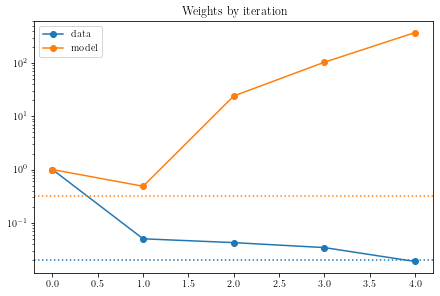
\includegraphics{img/dtvariant_weights.png}
\caption{Weights for each iteration, solving \(H_{\Delta t}\)}
\end{figure}

Iteration 0 seems slightly overfit, due to the oscillations in the
estimate at small time in \(S\). By iteration 2, the fit is already
degraded, and by iteration 3, the estimate is very underfit.

\begin{figure}
\centering
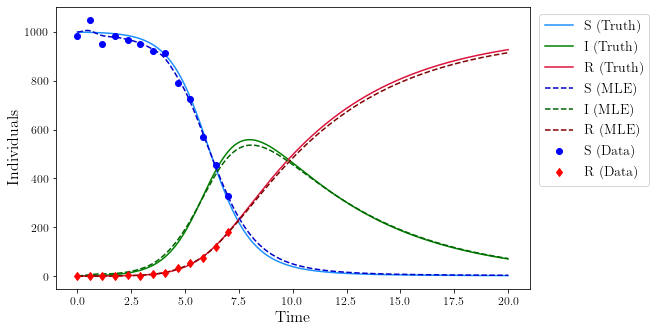
\includegraphics{img/dtvariant_fit_iter0.png}
\caption{Fit to \(H_{\Delta t}\) at iteration \(i=0\)
(\(\beta=1.21, \alpha=0.20\))}
\end{figure}

\begin{figure}
\centering
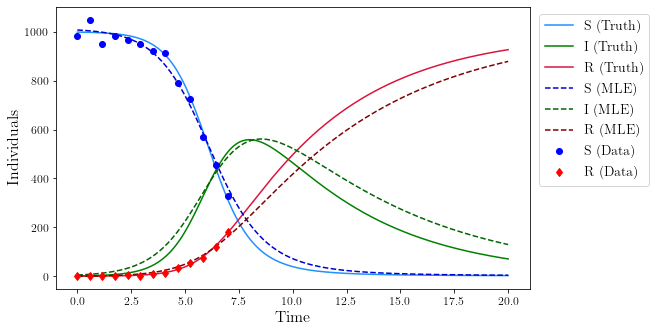
\includegraphics{img/dtvariant_fit_iter2.png}
\caption{Fit to \(H_{\Delta t}\) at iteration \(i=2\)
(\(\beta=1.00, \alpha=0.16\))}
\end{figure}

\begin{figure}
\centering
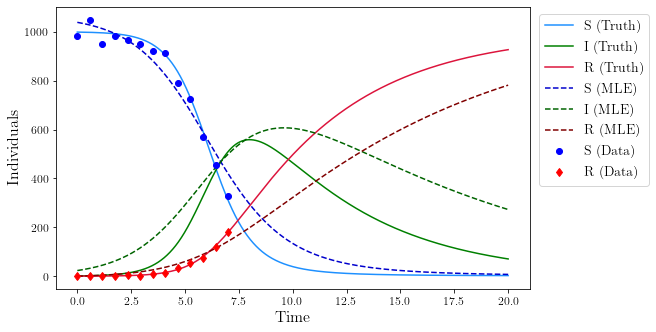
\includegraphics{img/dtvariant_fit_iter3.png}
\caption{Fit to \(H_{\Delta t}\) at iteration \(i=3\)
(\(\beta=0.70, \alpha=0.10\))}
\end{figure}

\hypertarget{balanced-variant}{%
\section{Balanced variant}\label{balanced-variant}}

Here, we fit the objective
\(H_{balanced} = -2\log \mathcal{L}_{balanced}\)

\[
H_{balanced} = \frac{1}{n}\lVert L(y - g(\Phi c))\rVert^2 + \frac{1}{m}\lVert W(D\Phi c - f(\Phi c, \theta)) \rVert^2 - 2\log{|L|} - 2\log{|W|}
\] where
\[L = \frac{1}{\sigma_L} \mathbb{I}\in \R_+^{n\times n},\qquad W = \frac{1}{\sigma_W} \mathbb{I} \in \R_+^{m\times m}\]
and we define the weights:
\[w = \left[\frac{1}{\sigma_L}, \frac{1}{\sigma_W}\right]\]

The idea of this balancing is to make the magnitudes of the two parts of
the objective function similar. Consider if \(m \to \infty\), i.e.~a
continuous integral. Then the objective function becomes dominated by
the model. Similarly, if we had an `infinite' amount of data, we would
force our function into interpolation, instead of ``smoothing''.

We find that in general, this leads to \emph{convergent} behaviour in
the weights, and thus convergence in the state/parameter estimates. This
may be because the two terms are similar in magnitude after the weight
update step of each iteration, meaning the objective is not weighted to
one term or the other.

\hypertarget{results-2}{%
\subsection{Results}\label{results-2}}

We use initial weights \([1, 1]\), and initial guesses
\(\sim \text{Poisson}(1000)\). We iterate for 10 iterations, which takes
25s. At the final iteration (\(i=9\)), we get a parameter estimate of
\(\beta = 1.0, \alpha=0.16\).

\begin{figure}
\centering
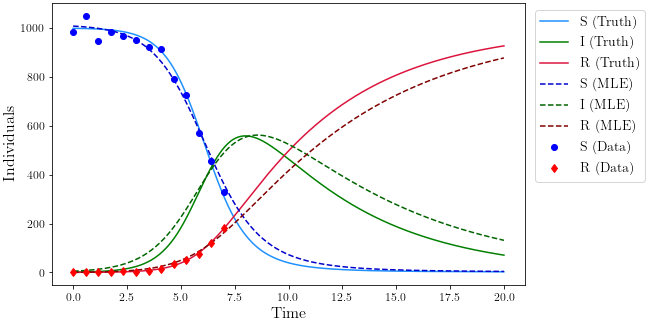
\includegraphics{img/balance_iter9.png}
\caption{Iteration \(i=9\) of \(H_{balanced}\) problem}
\end{figure}

We see that the weights converge, and approach some value (when plotted
in the weight-space).

\begin{figure}
\centering
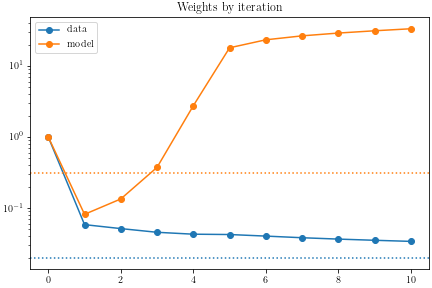
\includegraphics{img/balance_weight.png}
\caption{Weights at each iteration of the \(H_{balanced}\) problem}
\end{figure}

\begin{figure}
\centering
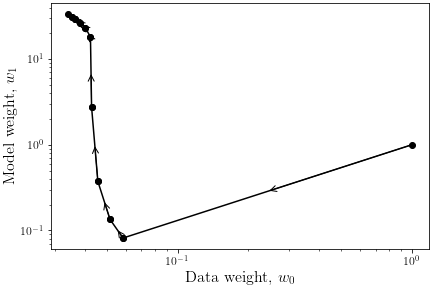
\includegraphics{img/balance_weight_space.png}
\caption{Weights in weight space at each iteration of the
\(H_{balanced}\) problem}
\end{figure}

We do see that the parameter estimate degrades after iteration \(i=4\),
and suspect this continues. This may suggest that the balancing is not
complete.

\hypertarget{balancing-with-delta-t-variant}{%
\section{\texorpdfstring{Balancing with \(\Delta t\)
variant}{Balancing with \textbackslash{}Delta t variant}}\label{balancing-with-delta-t-variant}}

We can combine balancing with \(\Delta t\) variant, to construct what
should be the `ideal' objective function.

\hypertarget{results-3}{%
\subsection{Results}\label{results-3}}

We see that when we start the initial weights at \([1,1]\), we do not
get the results we want. Examining the weights plot, we see that the
solution converges towards an interpolation-style fit. This suggests
that there are a large quantity of ``stable'' weights that the algorithm
can converge to
